\documentclass[12pt]{paper}

\usepackage{amsmath}
\usepackage{graphicx}

\begin{document}
% Setup
\section{Potential Fields}
\subsection{Setup}
The implementation of Potential Fields in Robocode went through a number of steps before coming to a satisfying conclusion. The implementation relies on a few assumptions that Robocode makes possible. First, Robocode always allows the robot get its exact $x$ and $y$ coordinates via \verb|getX()| and \verb|getY()| respectively. The heading of the robot can be gathered from a call to \verb|getHeading()|. The potential field implementations focus on manipulating the heading of the robot and the speed settings to get effective navigation and obstacle avoidance. Potential fields didn't require any special setup like the other methods tested, so jumping into the development was mostly painless.

% Experiments
\subsection{Experiments}
The first goal of potential field implementation was getting a simple proof of concept working in Robocode. The environment was unfamiliar, but fairly simple, so this didn't pose too great a problem. The initial tests were simple single agent environments with a stationary goal. To encode the notion of a ``goal'' in Robocode a stationary bot was used. To calculate the angle of rotation needed to point towards the goal, the robot coordinates and goal coordinates were subtracted and passed to the arctangent variant \verb|Math.atan2()|. This could be used to modify the current heading value, and thus turn the robot towards the goal. 

While the initial tests worked, the performance was less than stunning. The simple motion model in Robocode was used as opposed to the advance, which meant that all the robot actions blocked. For this simple example it didn't pose much of a problem, but it made scaling the speed as the bot approached the goal less than ideal. It did cause problems in later tests and would eventually be changed.

The next reasonable step seemed to use a moving goal since a stationary goal wasn't especially interesting to watch. Again, as with all the tests, a simple robot was used to implement the goal. It was coded to follow a simple pattern around the environment as quickly as possible. The test robot would rotate in a circle until it located the goal. Once the goal was found, it would do its best to continue heading towards the goal. 

It was this test that made it evident that the simple motion model wasn't sufficient. While tasks like sweeping the radar can be performed in the simple model, they eat up ticks that the robot could spend doing something else. The bot would end up rotating the radar for one tick, then turning with another tick, and then moving forward with yet another tick. 

\begin{figure}[htb]
\centering
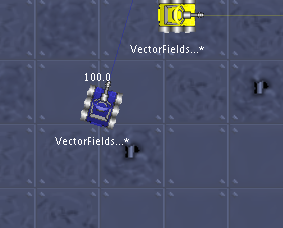
\includegraphics[width=0.5\textwidth]{images/SimpleRadarFailure}
\caption{Notice that the blue robot has lost track of the goal and is tracking an older position.}
\end{figure}

In an effort to save ticks and make the motion of the robot smoother, the radar was locked facing forward so the bot would always scan the direction it faced. However, the bot would sometimes lose track of the goal if it passed to close or made sudden direction changes. In addition, because the actions in the simple motion model block, the speed had to be set to the lowest possible setting. If it wasn't, the robot would attempt to move forward some number of units in the environment before doing another radar sweep. This resulted in the robot losing track of the goal quite quickly. So the decision ended up being between extremely slow motion that eventually lost track of the goal, or slightly faster motion that quickly lost track of the goal. Either way, these results weren't satisfying and it was evident that a new approach was needed.

After doing some research, it was decided that the advanced motion model was needed to improve the implementation. Unfortunately the examples and tutorials provided for Robocode only touch on the simple motion model. With a bit of persistence the model was understood enough for implementation. Instead of actions blocking, the robot queues up actions until a call to \verb|execute()| or \verb|scan()| is encountered. Then it attempts to execute all the queued commands simultaneously while obeying the physics of the environment. 

The initial test of the advanced motion model used a moving goal. In order to minimize the amount of time the robot spent following the old position of the goal, the radar was constantly rotated at maximum speed independent of the position and heading of the bot. This allowed for much improved performance. The robot's speed could be increased quite a significant amount without worry that it would overshoot and hit the goal or lose track of its location. That being said, the motion of the tracking robot was not perfect. There was often a delay in recognizing the changing position of the goal. 

The main issue was the wasted ticks sweeping the radar through empty space. This would cause the robot to track old positions while the radar completed its sweep. What was needed was a perfect radar lock so that the robot would always have the exact position of the goal. While the performance with the sweeping radar was satisfactory, it was felt that perfecting the situation where there weren't obstacles would only make future implementations easier and cleaner.

\begin{figure}[htb]
\centering
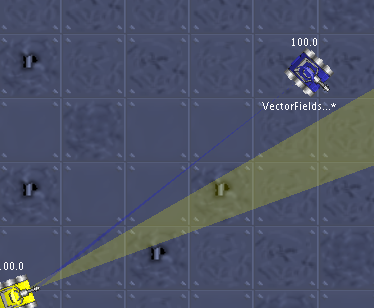
\includegraphics[width=0.5\textwidth]{images/RadarLock}
\caption{The blue tracking robot has located the goal with its radar, even though it is facing a different direction. It will never lose track of the goal now that it has a lock.}
\label{Radar Lock Example}
\end{figure}

To implement a radar lock that would never slip required simple algebraic manipulation of the state information present when a onScannedRobot event occurred. Whenever the goal was scanned, the radar's rotation was set to the tracking robot's heading added to the scanned ``goal'' robot's heading minus the radars heading. More succinctly, $NewRadarHeading = RobotHeading + GoalHeading - CurRadarHeading$. This angle was then normalized so that it fell within the range of $[-\pi, \pi]$. This caused the radar to constantly rotate towards the direction that the goal was navigating so the radar never slipped and the goal was never lost. It also minimized the amount that the radar needed to be rotated so that less ticks were spent uselessly spinning the radar.

Performance with the radar lock implemented was near as perfect as the simulation would allow. The robot could travel just as fast as the goal and never lose track of the location. In fact, the max speed of the tracking robot had to be turned down to ensure that it didn't catch up to and crash into the goal. In addition, because the tracking was so smooth, the speed of the bot could be appropriately scaled based on distance to the goal without fear of any blocking actions causing a loss of the goal or a slow scan resulting in a crash.

Once the moving goal tracking had been sufficiently implemented, the next obvious step was obstacle avoidance. As with the goal, obstacles were nothing more than stationary or moving robot entities added to the simulation. The initial implementation of obstacle avoidance was simplified to include a single stationary obstacle and a stationary goal. This ensured that all issues with obstacle avoidance could be ironed out before dealing with the issues of adding a moving goal to the equation. 

When a robot was scanned by the tracking robot that wasn't recognized as the goal, the robot would calculate and save the coordinates of that bot and assume it was an obstacle. Goal or obstacle recognition was handled in the onScannedRobot event handler by accessing the scanned object's name. The appropriate name values were simply coded into constants and checked whenever something was scanned.

Since the location of the obstacle was stored as a pair of coordinates, the distance from the robot to the obstacle could be calculated during each iteration of the navigation loop. This distance value was checked against a previously defined threshold value that determined if the navigating robot was within the area of affect of the obstacle. The formula used to determine the repulsion from the obstacle was $\frac{Range - calcDist}{Range} * MaxSpeed$ where $Range$ was the threshold distance for the obstacle and $calcDistance$ was the calculated distance from the robot to the obstacle. $MaxSpeed$ was the maximum speed that the robot could be set to when running. This formula returned the amount that the robot's speed should be adjusted based on its location relative to the obstacle. This effectively slowed the robot down as it neared obstacles, which was necessary to ensure that it wouldn't cause a collision due to excessive speed in tight quarters. The direction of the repulsion vector was done using the \emph{archtangent} function like the goal implementation, except that the direction is from the obstacle to the robot so the ``force'' is repulsive.

The next step was implementing a moving goal along with obstacle avoidance. Like the previous version with the stationary obstacle, the perfect radar lock could not be used because the tracking robot needed to scan for obstacles. Because it was planned that moving obstacles would be added in the future, a constantly rotating radar was used. While this may waste space over-rotating the radar, the trade off of perfect information for added situational awareness was both necessary and worthwhile. 

While the motion of the tracking robot was not nearly as smooth when a perfect lock was not used, the performance was still quite good. The motion was slightly jerky since a number of ticks pass before updating the goal position, but the obstacle avoidance worked well and the robot navigated cleanly.

As a final test for potential fields, a reasonably complicated scenario with multiple obstacles, both moving and stationary, and a moving goal was constructed. Multiple obstacles meant that the code needed to be adjusted to handle the vector calculations in a general way. Because all the bots in the simulation could be given unique names by changing the class names in the implementation files, it was decided that a HashMap that mapped the robot names to instances of a class Enemy that held location data would be an efficient method for handling an unknown number of obstacles. 

\begin{figure}[htb]
\centering
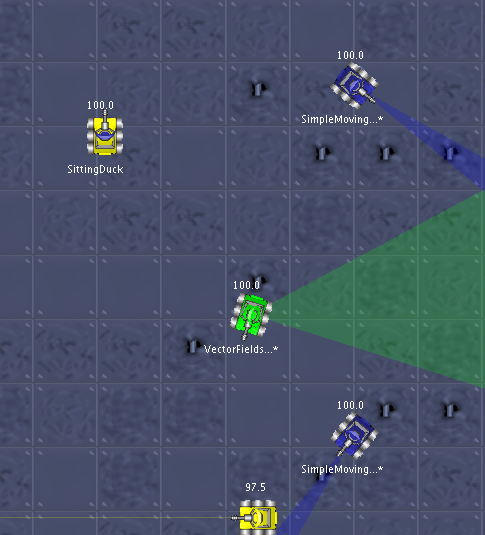
\includegraphics[width=0.8\textwidth]{images/FinalRun}
\caption{The final test for the Potential Field implementation features obstacles, both stationary and moving, and a moving goal.}
\label{Radar Lock Example}
\end{figure}

Each time the goal or an obstacle was scanned, onScannedRobot would grab the scanned objects name and insert an instance of the Enemy class into the HashMap. The Enemy class holds the calculated coordinate pair for the location of the scanned item as well as it's bearing at the time of the scan. The bearing was not used, but it was stored in case future modifications needed the additional information. This HashMap could then be iterated through in the navigation loop and the vectors could be calculated appropriately.

The potential fields implementation handled the course beautifully. When it would pass between obstacles, its speed would be dropped sufficiently to avoid any near collisions. It also handled the moving obstacle quite well, so long as the obstacle buffer was set sufficiently high. If it was set too low, often times the robot would not react in time to sudden directional changes from the obstacles and would be crashed into. 

Perhaps the only change I would make to this algorithm would be taking into consideration how much to scale the speed based on how many obstacles are affecting the tracking robot. Each drop in speed was calculated independently for each obstacle. So if the robot was within range of three obstacles, each one of those obstacles would cause its own drop in the tracking robot's speed. This meant that often times the robot's speed would drop significantly even if it wasn't especially close to any one obstacle. However, the performance was still quite smooth with the current implementation.

To finalize potential fields, it was decided that noise needed to be added to the model. Comparison really wouldn't be fair with the other methods if potential fields operated solely in an ideal environment. Noise was added in two ways. The first method added a random offset to the turning angle at a certain probability. As an example, twenty percent of the time the robot would slip $\pm 30^{\circ}$ when turning. The second method added small amounts of noise to the radar scans by adding or subtracting some $\epsilon$ from the calculated coordinate pair of the obstacle or goal.

The potential fields implementations handled the noise quite well. The slips, even when really large, did not impact the results nearly as much as expected. Mostly the navigation path got a bit jittery, but the results were never catastrophic. Similarly, the robot didn't have too difficult of a time handling the radar noise. The noise was fairly small in comparison to the range of the obstacles, so there were not any collisions as a result of this. The only time the radar scan noise caused any truly noticeable affects was when the noise was turned up extremely high. So long as the noise was reasonable--$\pm$ a few percent of the total distance to the object--then the effect was not significant enough to cause problems.

% Conclusion
\subsection{Conclusion}
Overall, the potential fields implementation handled the majority of the situations it was put into quite well. Initially, the simple implementation worked as a proof of concept but not much else. It moved terribly slow, but it found the goal nonetheless. Moving over to a moving goal showed the weaknesses present in the simple motion model. It made it hard to constantly follow the moving goal. In fact, it was pretty much guaranteed that the tracking would fail unless the robot was started in the middle of the course and the goal robot travelled a specific path. Additionally, the speed of the tracking robot couldn't be scaled with regards to its distance from the goal without running the risk that it would lose track of the goal.

The advanced motion model helped to smooth out the performance and addressed the issues made evident in the simple model tests. The radar locking experiment shows what the robot was capable of when it had perfect knowledge, and it showed the smoothest results when just dealing with a goal and no obstacles. It also demonstrated the speed adjustment with regards to distance from the goal best since it had perfect information on the goal. 

The obstacle avoidance results were quite good after the discovery of the advanced motion model. At first, expectations were low when watching the test runs with the simple motion model. However, the performance took off with the advanced motion model. Tracking a goal while dealing with an object was no challenge for the test bots. Even a moving goal with moving and stationary obstacles worked quite well.

Even with all the successes, there were still problems present with the method. The implementations had difficulty with congested environments, especially when it would attempt obstacle avoidance too near to a wall. This was especially evident with high \emph{MaxSpeed} settings. Often times the robot would sweep wide around an obstacle that was near a wall and collide. Unfortunately, with Robocode it isn't possible to detect the wall with the radar. It would be possible to simply generate a repulsive vector based on the coordinates of the robot with regards to the width and height of the arena; But that seemed a bit like cheating. Abusing the perfect world coordinates to the extent of making up readings didn't seem in the spirit of the tests.

Additionally, the method struggled with closely placed obstacles since it couldn't detect the optimal path around them. This is where the planning of the other methods could become beneficial. The reactionary behaviour of the potential fields could be used to subsume the long term thought out behaviour present in the alternative methods. This could create quite a robust system.

% This is for the final conclusion 
Potential Fields performed quite well in the Robocode environment. Combining the advanced motion model with the potential fields approach allowed for smooth navigation and obstacle avoidance. The potential fields method was quite robust and handled changes to the environment the easiest. The primary limiter for performance was the ability to scan the environment fast enough with the radar sweeps. The navigating bot's max speed and obstacle avoidance radius had to be tuned with the radar in mind. Even so, the robot was able to navigate fairly complex environments. Ob course, that isn't to say that potential fields didn't have problems. Suboptimal navigation is always an issue that potential fields will have. This became especially true when obstacles were placed really close to the wall since the radar sweeps didn't read the distance to the walls. It would also rather avoid close obstacles than navigate between tight paths, which may not always be optimal. There is also the issue of local minima causing navigational issues. That being said, potential fields handled the environment quite well.
\end{document}
